\section{Overview}
 
The {\tt CLAS12} detector will be located in experimental Hall B. It 
will replace the {\tt CLAS} detector and re-use many systems, including 
magnets, beam line components, cryogenic targets, support structures, and 
some particle detectors. The planned {\tt CLAS12} detector is shown in 
Fig.\ref{in_clas}.

%%%%%%%%%%%%%%%%%%%%%%%%%%%%%%%%%%%%%%%%%%%%%%%%%%%%%%%%%%%%%%%%%%%%%%
\begin{figure}[htbp]
\centering
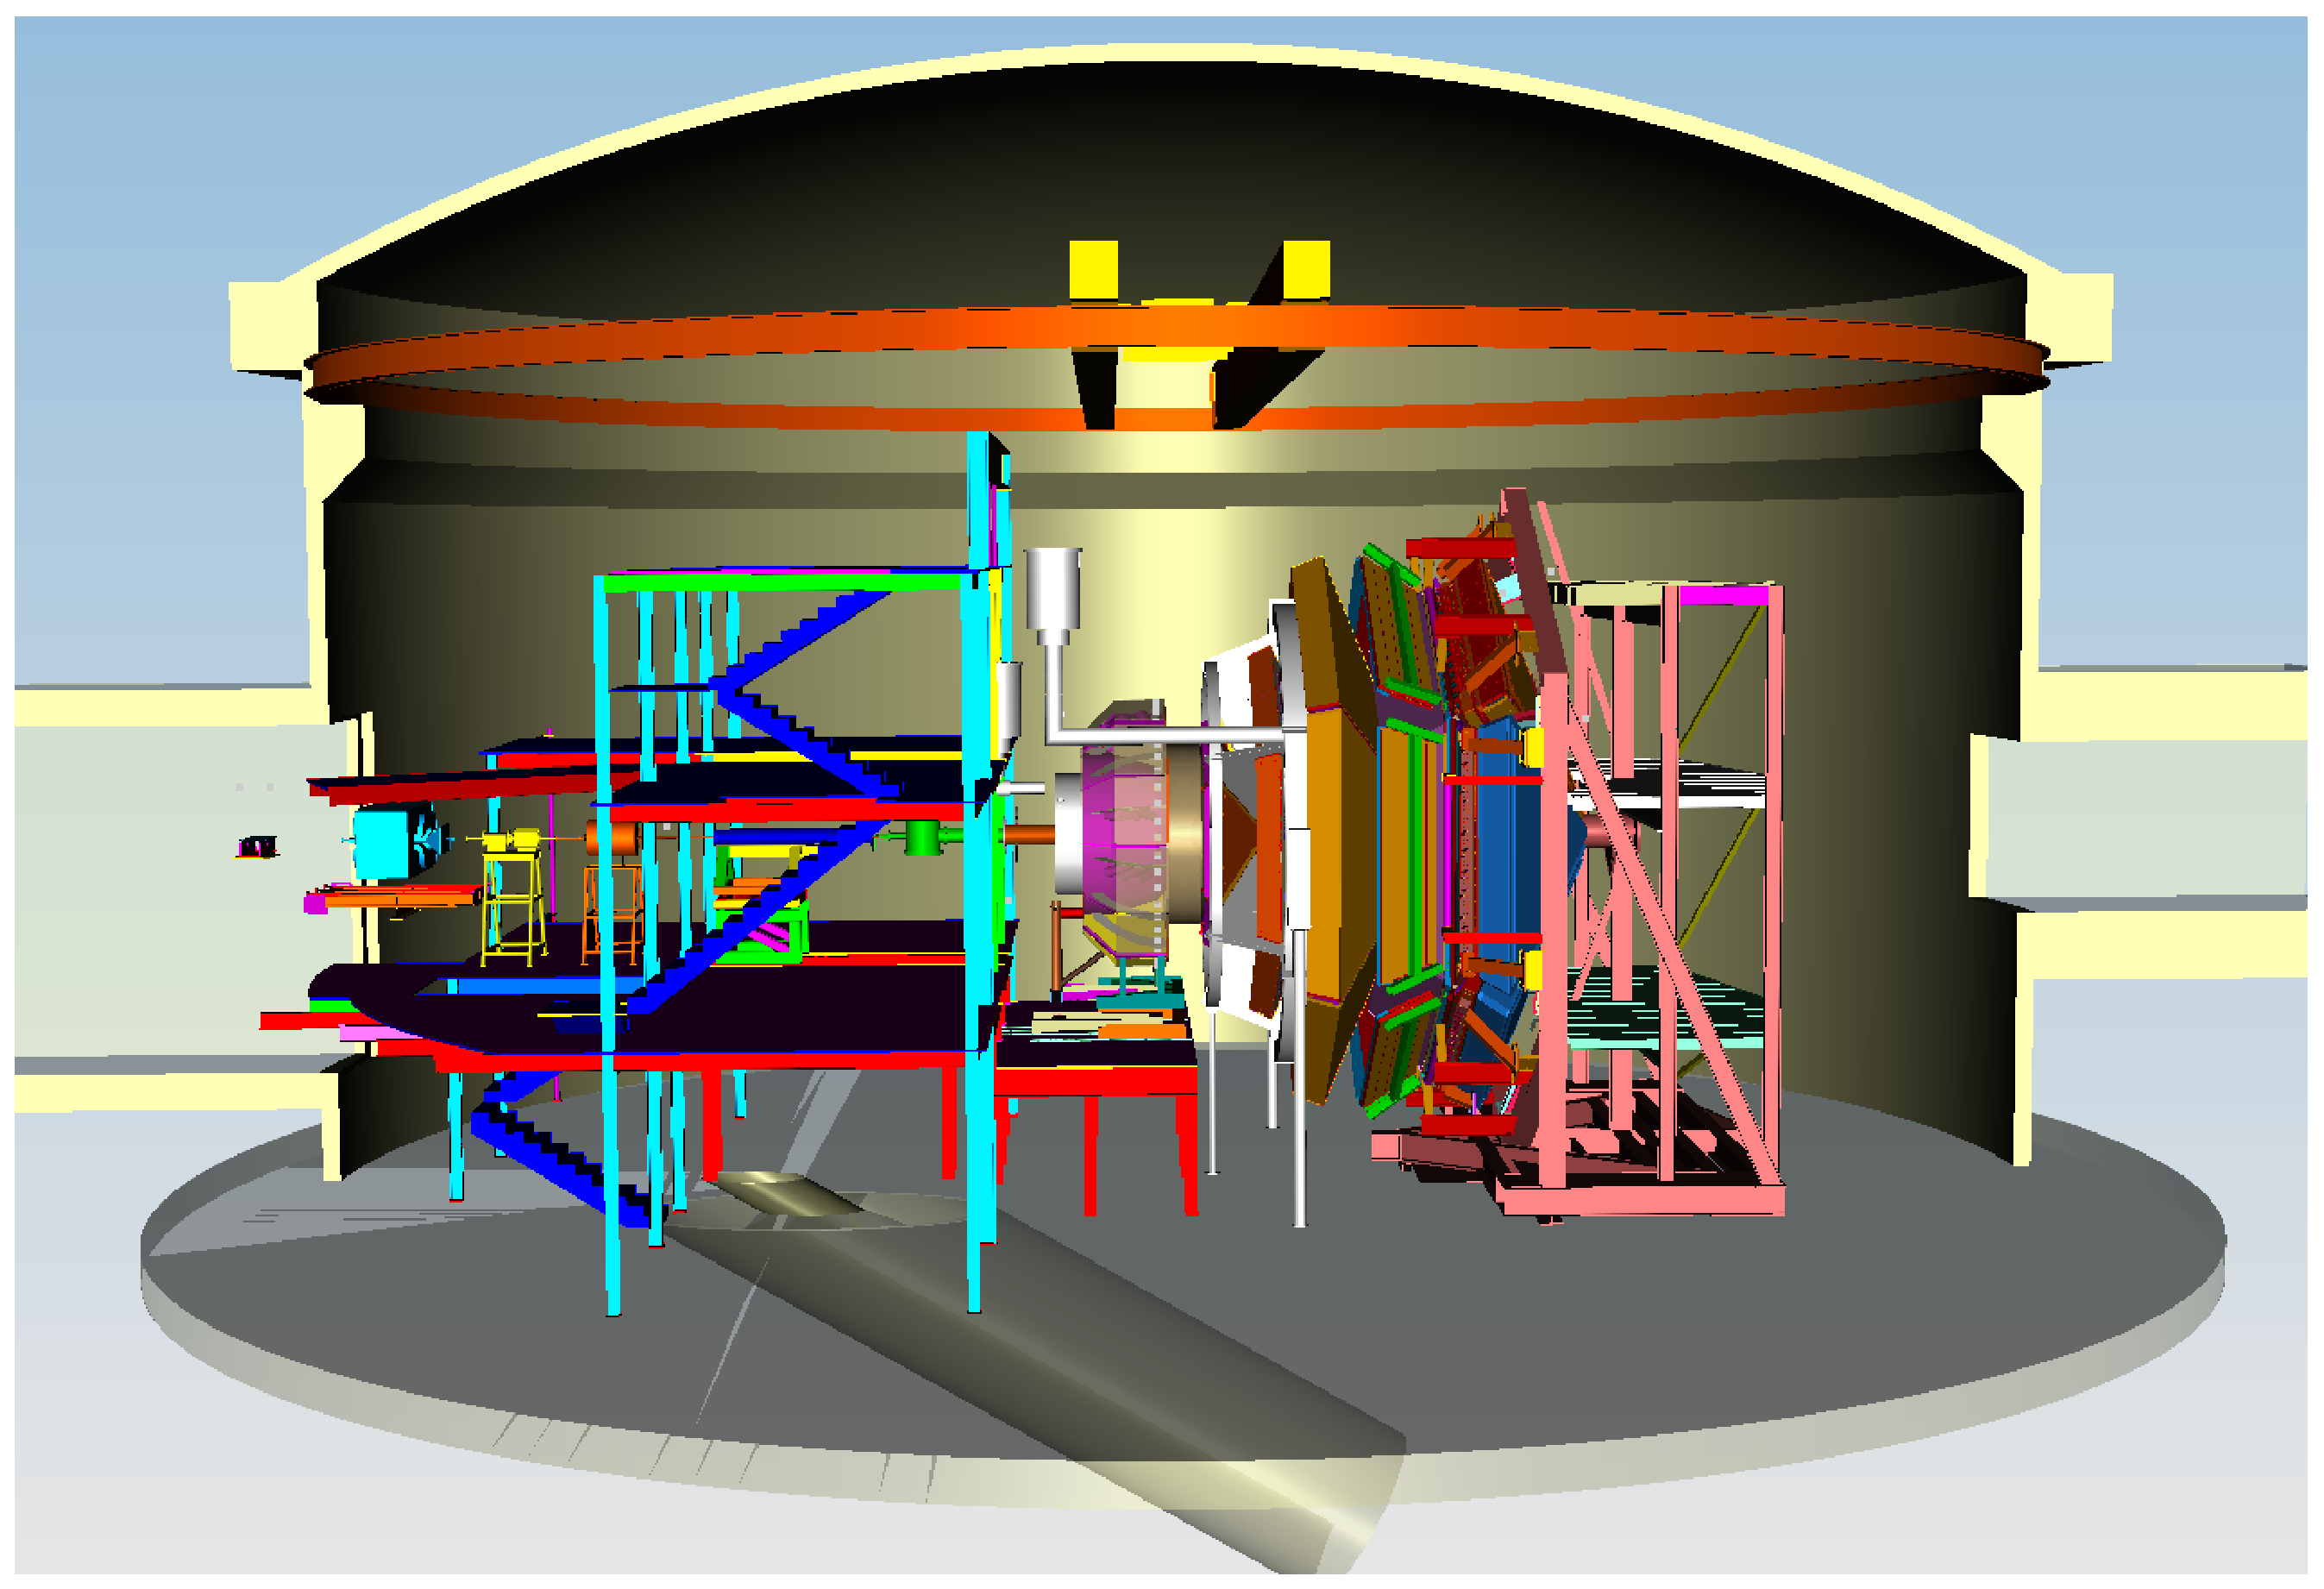
\includegraphics[width=0.6\textwidth]{fig1overall.eps}
\caption{\small{Model of the {\tt CLAS12} detector in Hall B.}}
\label{in_clas}
\end{figure}
%%%%%%%%%%%%%%%%%%%%%%%%%%%%%%%%%%%%%%%%%%%%%%%%%%%%%%%%%%%%%%%%%%%%%%

Two of the major structures in Hall B will be retained.  The first is
the ``Space Frame", the structure on the left side of Fig.~\ref{in_clas},
and the second is the Forward Carriage shown on the right side of the 
figure.  The Space Frame is a fixed-deck structure, while the Forward 
Carriage, which is movable, is a large structure that supports detectors, 
cables, and instrumentation racks, and weighs approximately 300~tons.  Some 
modifications will be required for each structure.  Major utilities and 
their distribution systems including electrical power, HVAC, cooling water, 
and cryogenics that currently service {\tt CLAS}, will be re-used for 
{\tt CLAS12}.  Shown in Fig.~\ref{in_clas} is the 20~ton polar crane.  
This crane has enough capacity to install all of the new components for 
{\tt CLAS12}.  Not shown for simplicity are all of the magnet power 
supplies, electronics racks for detector signal processing and device 
controls, cable trays, and the handrails on the decks.

\section{Permanent Platforms}

There are four large frame structures in Hall B. Two of which will be 
re-used for {\tt CLAS12}. The largest structure is fixed in position to 
the Hall and called the Space Frame. The other structure we will re-use 
is the Forward Carriage. It is not fixed in location and must be moved 
downstream to allow detector installation and maintenance. 

\subsection{Space Frame}
\label{sec:in_sf}

The largest structure in Hall B is the Space Frame shown in Fig.~\ref{in_sf}. 
The Space Frame has three levels, with the electron beam passing between 
Levels~1 and 2.  Level~1 has a set of rails that allow beam line components 
to be located at various $z$ locations along the beam. 

%%%%%%%%%%%%%%%%%%%%%%%%%%%%%%%%%%%%%%%%%%%%%%%%%%%%%%%%%%%%%%%%%%%%%%
\begin{figure}[htbp]
\centering
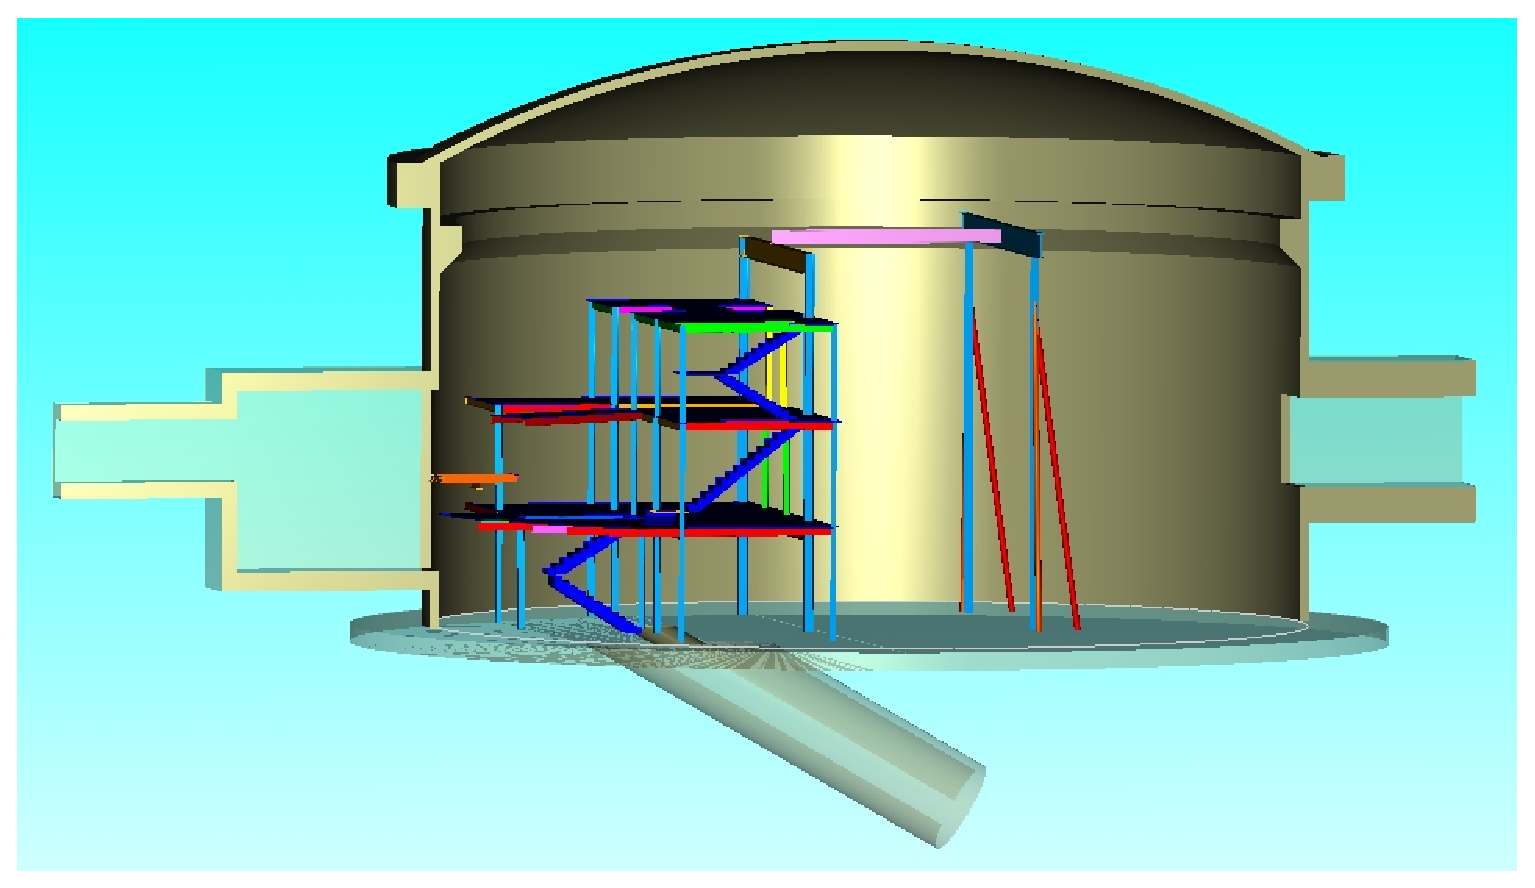
\includegraphics[width=0.6\textwidth]{fig2spaceframe.eps}
\caption{\small{View of Hall B without any of the detector elements or
the Forward Carriage to highlight the layout of the Space Frame.  This
figure shows the existing configuration existing in Hall~B.}}
\label{in_sf}
\end{figure}
%%%%%%%%%%%%%%%%%%%%%%%%%%%%%%%%%%%%%%%%%%%%%%%%%%%%%%%%%%%%%%%%%%%%%%

Some modifications to the Space Frame are anticipated, which include:

\begin{itemize}

\item removal of the downstream structure and the top beam;
\item a deck structure (called Sub-level~1) will be added to support the 
      HTCC and solenoid (see Fig.~\ref{in_htcc});
\item Level~2 will have the deck cut out above the beam line to allow the 
      solenoid magnet to move upstream;  
\item a small raised platform may be required to access the cryogenic 
      distribution can. 
\end{itemize}

%%%%%%%%%%%%%%%%%%%%%%%%%%%%%%%%%%%%%%%%%%%%%%%%%%%%%%%%%%%%%%%%%%%%%%
\begin{figure}[htbp]
\centering
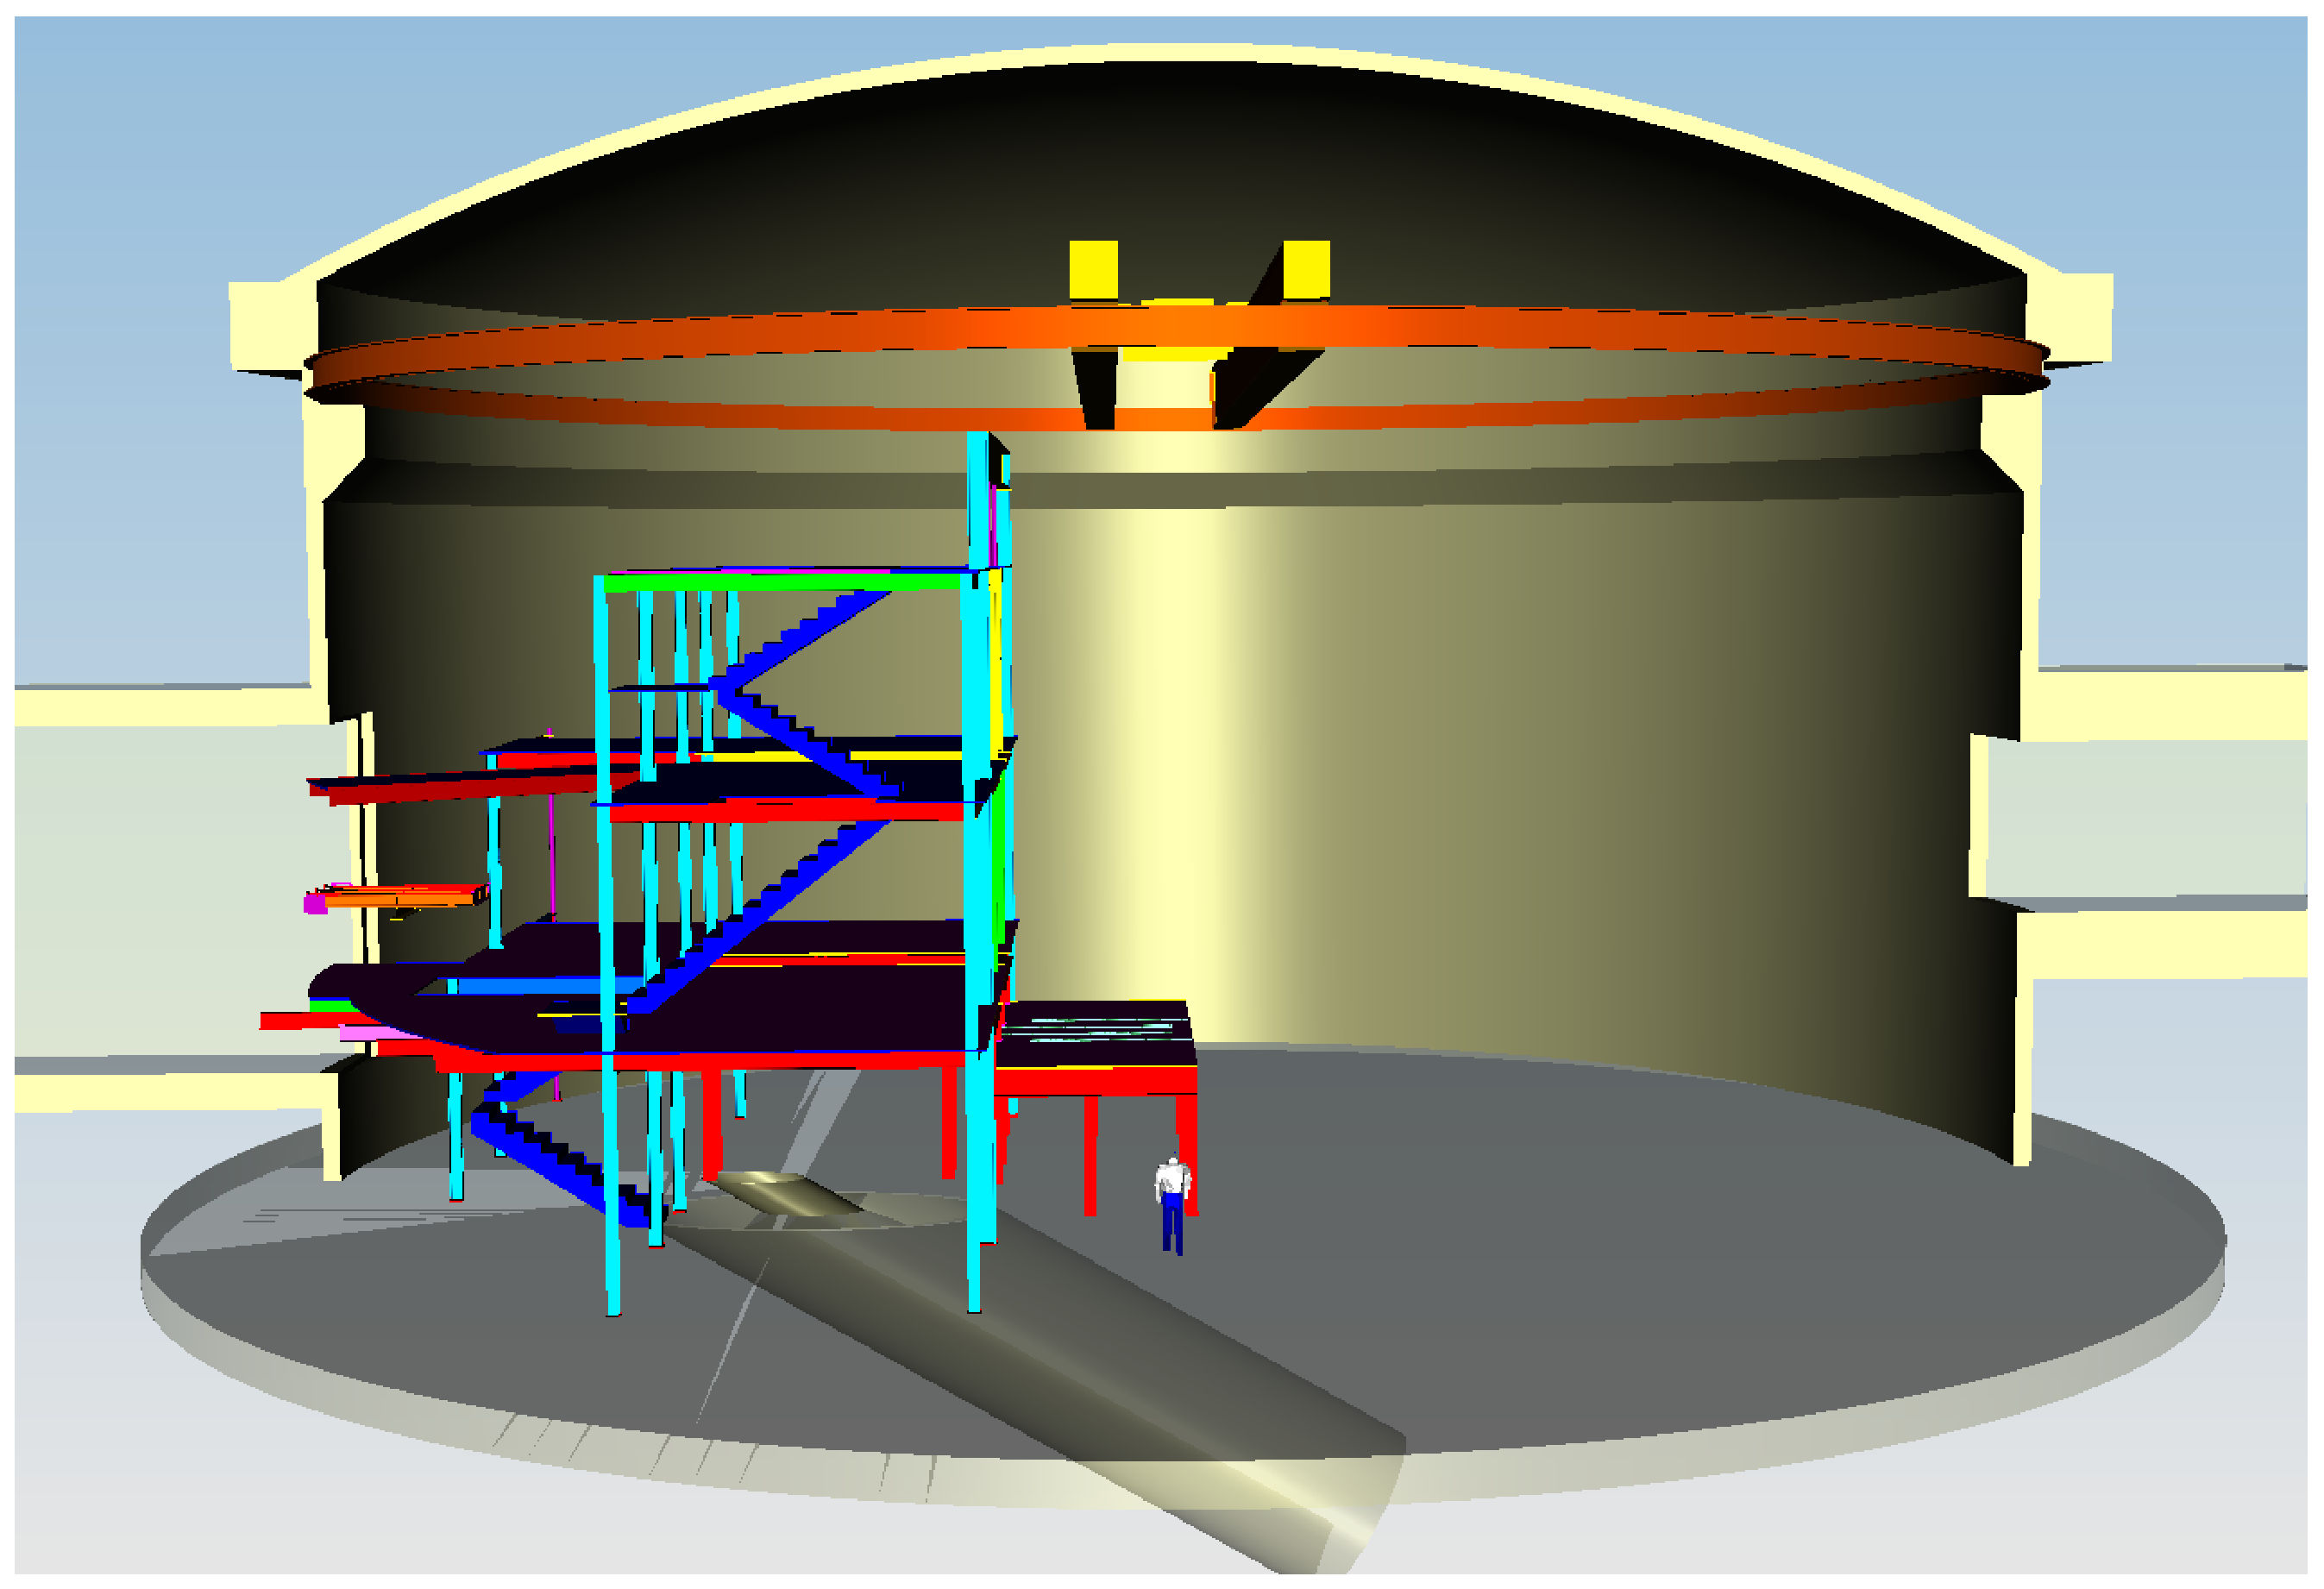
\includegraphics[width=0.6\textwidth]{fig4sf_deck.eps}
\caption{\small{View of the Space Frame as modified for {\tt CLAS12} 
showing the addition of the Sub-level~1 deck for the HTCC and solenoid.
Also shown is the cut-out for the solenoid on Level~2.}}
\label{in_htcc}
\end{figure}
%%%%%%%%%%%%%%%%%%%%%%%%%%%%%%%%%%%%%%%%%%%%%%%%%%%%%%%%%%%%%%%%%%%%%%

\subsection{Forward Carriage}

The Forward Carriage currently supports 200,000~lbs of calorimeters,
10,000~lbs of TOF, 15,000~lbs of LTCC, and roughly 15,000~lbs of delay 
cables and electronics (see Fig.~\ref{in_fc}).  The carriage was weighed 
using hydraulic jacks and the total was approximately 600,000~lbs. The 
{\tt CLAS12} upgrade will include adding the following to the Forward 
Carriage: 

\begin{itemize}
\item six pre-shower calorimeter modules (PCAL) weighing 70,000~lbs;
\item a second layer of forward time-of-flights (FTOF) panels weighing 
12,000~lbs;
\item a set of large-angle time-of-flight panels (panel~2) weighing 
6,000~lbs.  
\end{itemize}

These additional loads may require strengthening of this carriage.  A 
finite element analysis of the carriage is being performed.  The results 
will be analyzed to determine what work will be required.

%%%%%%%%%%%%%%%%%%%%%%%%%%%%%%%%%%%%%%%%%%%%%%%%%%%%%%%%%%%%%%%%%%%%%%
\begin{figure}[htbp]
\centering
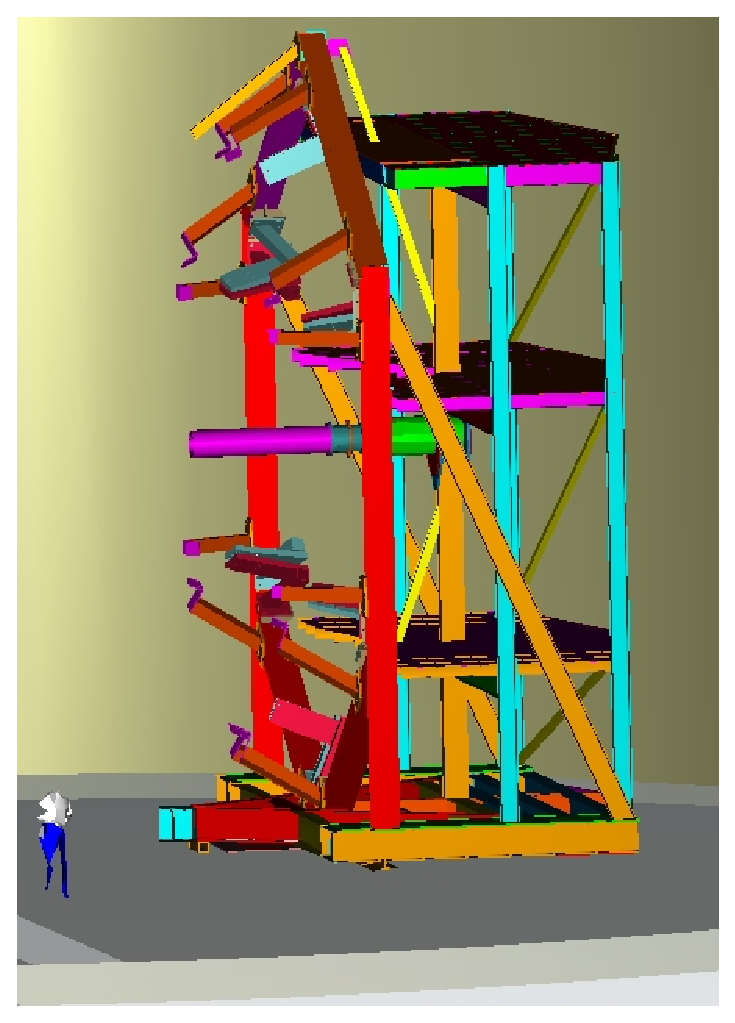
\includegraphics[width=0.6\textwidth]{fig5fc.eps}
\caption{\small{Forward Carriage in Hall B with all detectors removed.}}
\label{in_fc}
\end{figure}
%%%%%%%%%%%%%%%%%%%%%%%%%%%%%%%%%%%%%%%%%%%%%%%%%%%%%%%%%%%%%%%%%%%%%%

\section{Tooling for Detector Installation and Maintenance}

Tooling for detector installation and maintenance was a major challenge 
for the {\tt CLAS} detector and will be again for {\tt CLAS12}. The 
addition of several new detectors and the increased thickness of the drift 
chambers will impose new constraints on accessing each of the detectors. 
The fact that all of the forward detectors are planer could make some of 
the installation tooling simpler. All tooling will be designed to facilitate 
safe installation and maintenance. Tooling that will carry loads will be 
tested to 125\% of the rated load. Equipment installation will be guided by 
principles from the EHS\&Q manual (Section~6000) and appropriate subsections.
Hazard analysis will follow the guidelines in Section~3210 of the EHS\&Q
manual.  In most cases, specific procedures will be developed and followed 
to assure worker and detector safety.  These procedures will be ``living'' 
documents and updated as new ideas are developed and processes tested that 
reduce the likelihood of equipment damage, reduce the possibility of 
personnel injury, or reduce the time required to carry out the work without 
sacrificing safety. 

\subsection{The HTCC Lifting Fixture}

The HTCC will be lifted to the beam line using the Hall~B polar crane.
The design of the detector will allow a single lift point with
minimal distance to the crane hook.  The total weight of the HTCC will
be around 5000~lbs. 

\subsection{Drift Chamber Tooling}

Drift chamber installation will require very specialized tooling.  These 
chambers are being designed to allow sectors to be installed and removed 
individually.  Due to the delicate nature of drift chambers, the handling 
and mounting systems must incorporate features that allow accurate placement
that impose only known loads.  The installation tooling must control the 
position carefully at all times.  The current design uses tooling that is 
similar in concept to the designs used in {\tt CLAS} for the LTCC (see
Fig.~\ref{cctool}).  The principle is that the detectors arrive in Hall~B 
on a truck or low-boy trailer.  A strong-back with a cantilever arm and
weight box will allow the individual drift chambers to be positioned near
their final positions, where they will be attached to their final
attachment linkages.  The strong-back is detached from the chamber and pulled 
back using the crane.  Final chamber positioning is done using some fine 
tuning adjustment screws that are attached to the torus cryostat.  

\subsection{Forward Time-of-Flight}

The FTOF system will have three panels mounted in each of the six
sectors of CLAS.  Panels-1a and 1b will be mounted in front of the 
PCAL and EC detectors, and panel-2 will be mounted off the side of the 
forward carriage.  Each TOF panel weighs about 2000~lbs.  The strong-back 
shown in Fig.~\ref{tofstrongback} was used for {\tt CLAS} and will be 
re-used for panel-1a mounting, and with modifications, for panel-1b 
mounting.  The panel-2 counters will be installed using the crane.

%%%%%%%%%%%%%%%%%%%%%%%%%%%%%%%%%%%%%%%%%%%%%%%%%%%%%%%%%%%%%%%%%%%%%%
\begin{figure}[htbp]
\centering
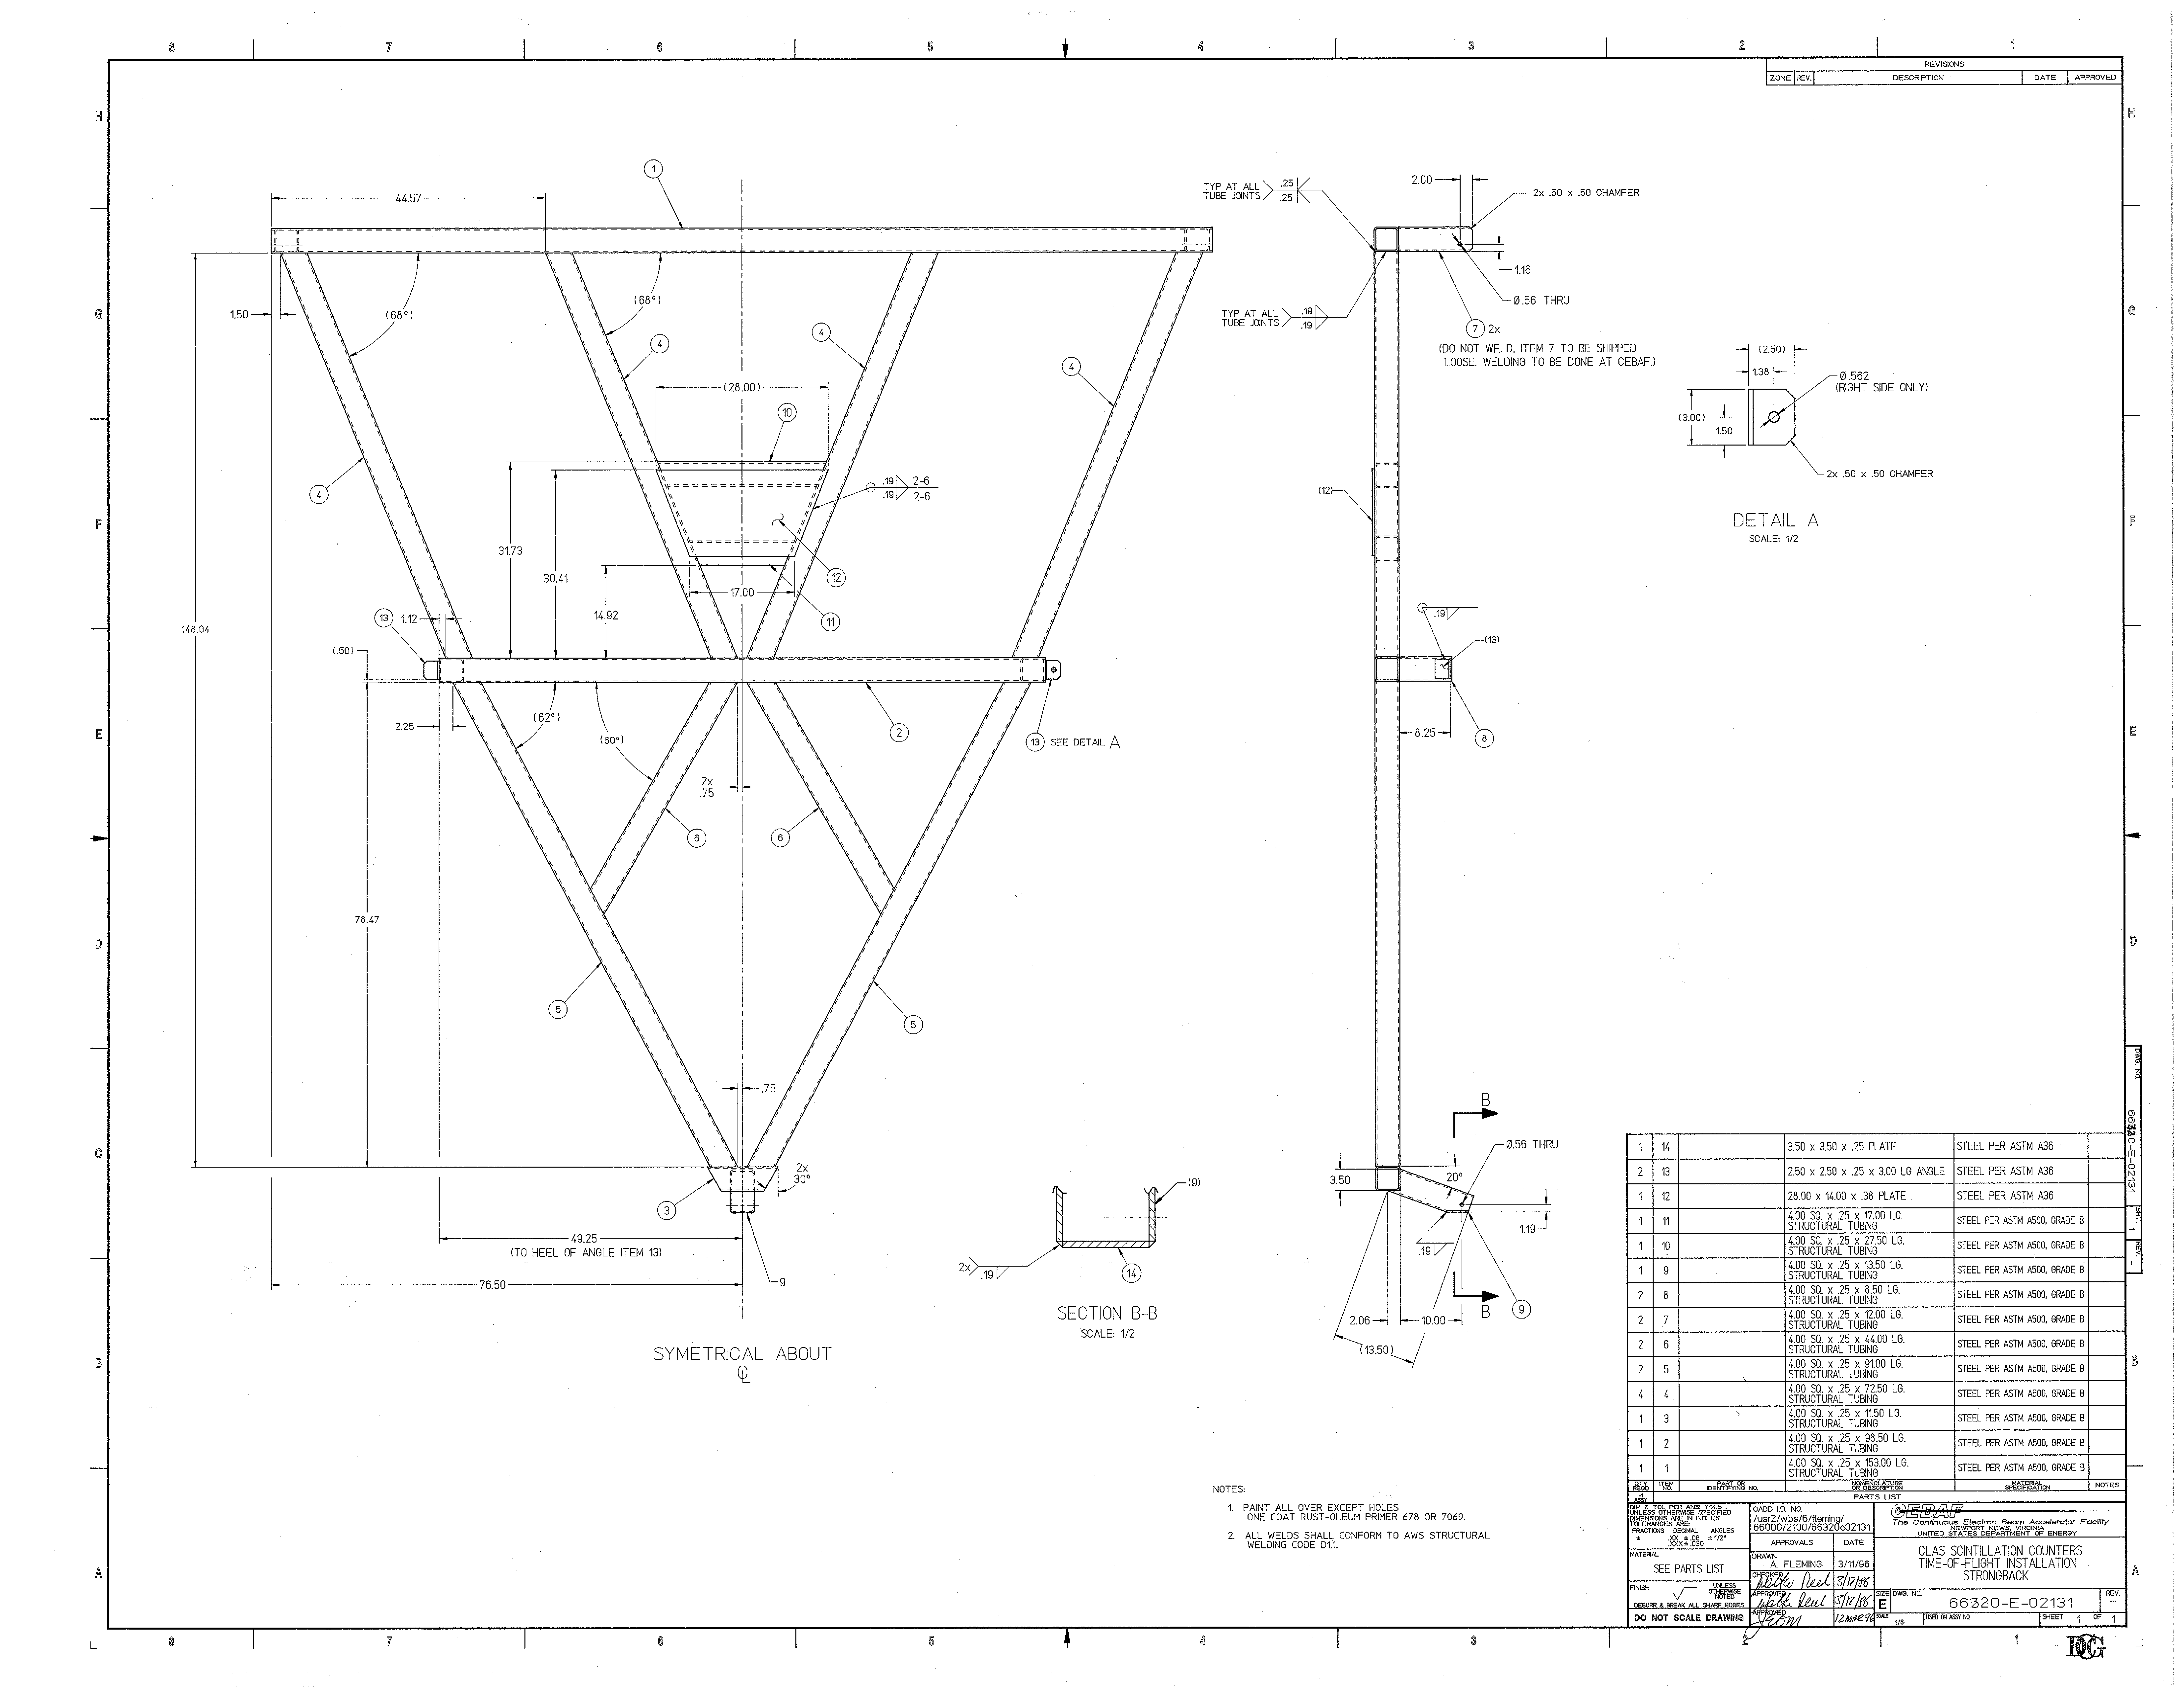
\includegraphics[width=0.6\textwidth]{ftof_strongback.eps}
\caption{\small{Engineering drawing of the FTOF strong-back assembly.}}
\label{tofstrongback}
\end{figure}
%%%%%%%%%%%%%%%%%%%%%%%%%%%%%%%%%%%%%%%%%%%%%%%%%%%%%%%%%%%%%%%%%%%%%%

\subsection{Low Threshold {\v C}erenkov Counter}

The LTCC will be modified slightly for {\tt CLAS12}.  The modifications 
include changing the optics and changing the side walls to make the 
detector upstream window flat.  Fig.~\ref{cctool} shows the lifting
fixture that currently exists for the LTCC, which may need modification 
because of reduced space in {\tt CLAS12}.

%%%%%%%%%%%%%%%%%%%%%%%%%%%%%%%%%%%%%%%%%%%%%%%%%%%%%%%%%%%%%%%%%%%%%%
\begin{figure}[htbp]
\centering
\includegraphics[width=0.6\textwidth]{ltcc_install.eps}
\caption{\small{Photograph of the LTCC lifting fixture as attached to
an existing LTCC sector in {\tt CLAS}.}}
\label{cctool}
\end{figure}
%%%%%%%%%%%%%%%%%%%%%%%%%%%%%%%%%%%%%%%%%%%%%%%%%%%%%%%%%%%%%%%%%%%%%%

\subsection{Pre-Shower Calorimeter}

The PCAL will be installed with tooling similar to the original EC 
tooling. It may even be possible to re-use the original tooling shown in
Fig.~\ref{ectool1} that was used for the {\tt CLAS} EC installation. 

%%%%%%%%%%%%%%%%%%%%%%%%%%%%%%%%%%%%%%%%%%%%%%%%%%%%%%%%%%%%%%%%%%%%%%
\begin{figure}[htbp]
\centering
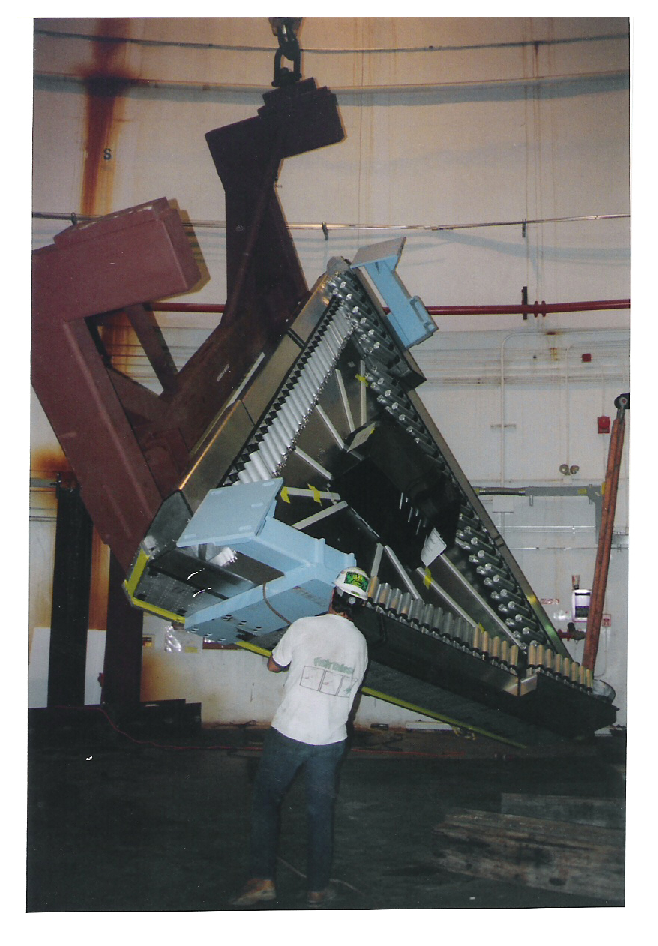
\includegraphics[width=0.6\textwidth]{ec_install.eps}
\caption{\small{Photograph of the EC tooling used to lift and install
the {\tt CLAS} EC sectors.}}
\label{ectool1}
\end{figure}
%%%%%%%%%%%%%%%%%%%%%%%%%%%%%%%%%%%%%%%%%%%%%%%%%%%%%%%%%%%%%%%%%%%%%%

\subsection{Solenoid}

The solenoid will be delivered to Hall B as a complete unit inside its 
cryostat.  The Hall~B crane will be used to lift the magnet to a cart that 
is waiting on Sub-Level~1 of the Space Frame.  A lifting bracket will 
be designed to match the magnet will be bolted to the magnet and used to 
allow a single point lift.  If the solenoid final weight is greater than
20~tons, a backup plan using a mobile 100~ton crane has been put in
place (see Fig.~\ref{mobile}).

%%%%%%%%%%%%%%%%%%%%%%%%%%%%%%%%%%%%%%%%%%%%%%%%%%%%%%%%%%%%%%%%%%%%%%
\begin{figure}[htbp]
\centering
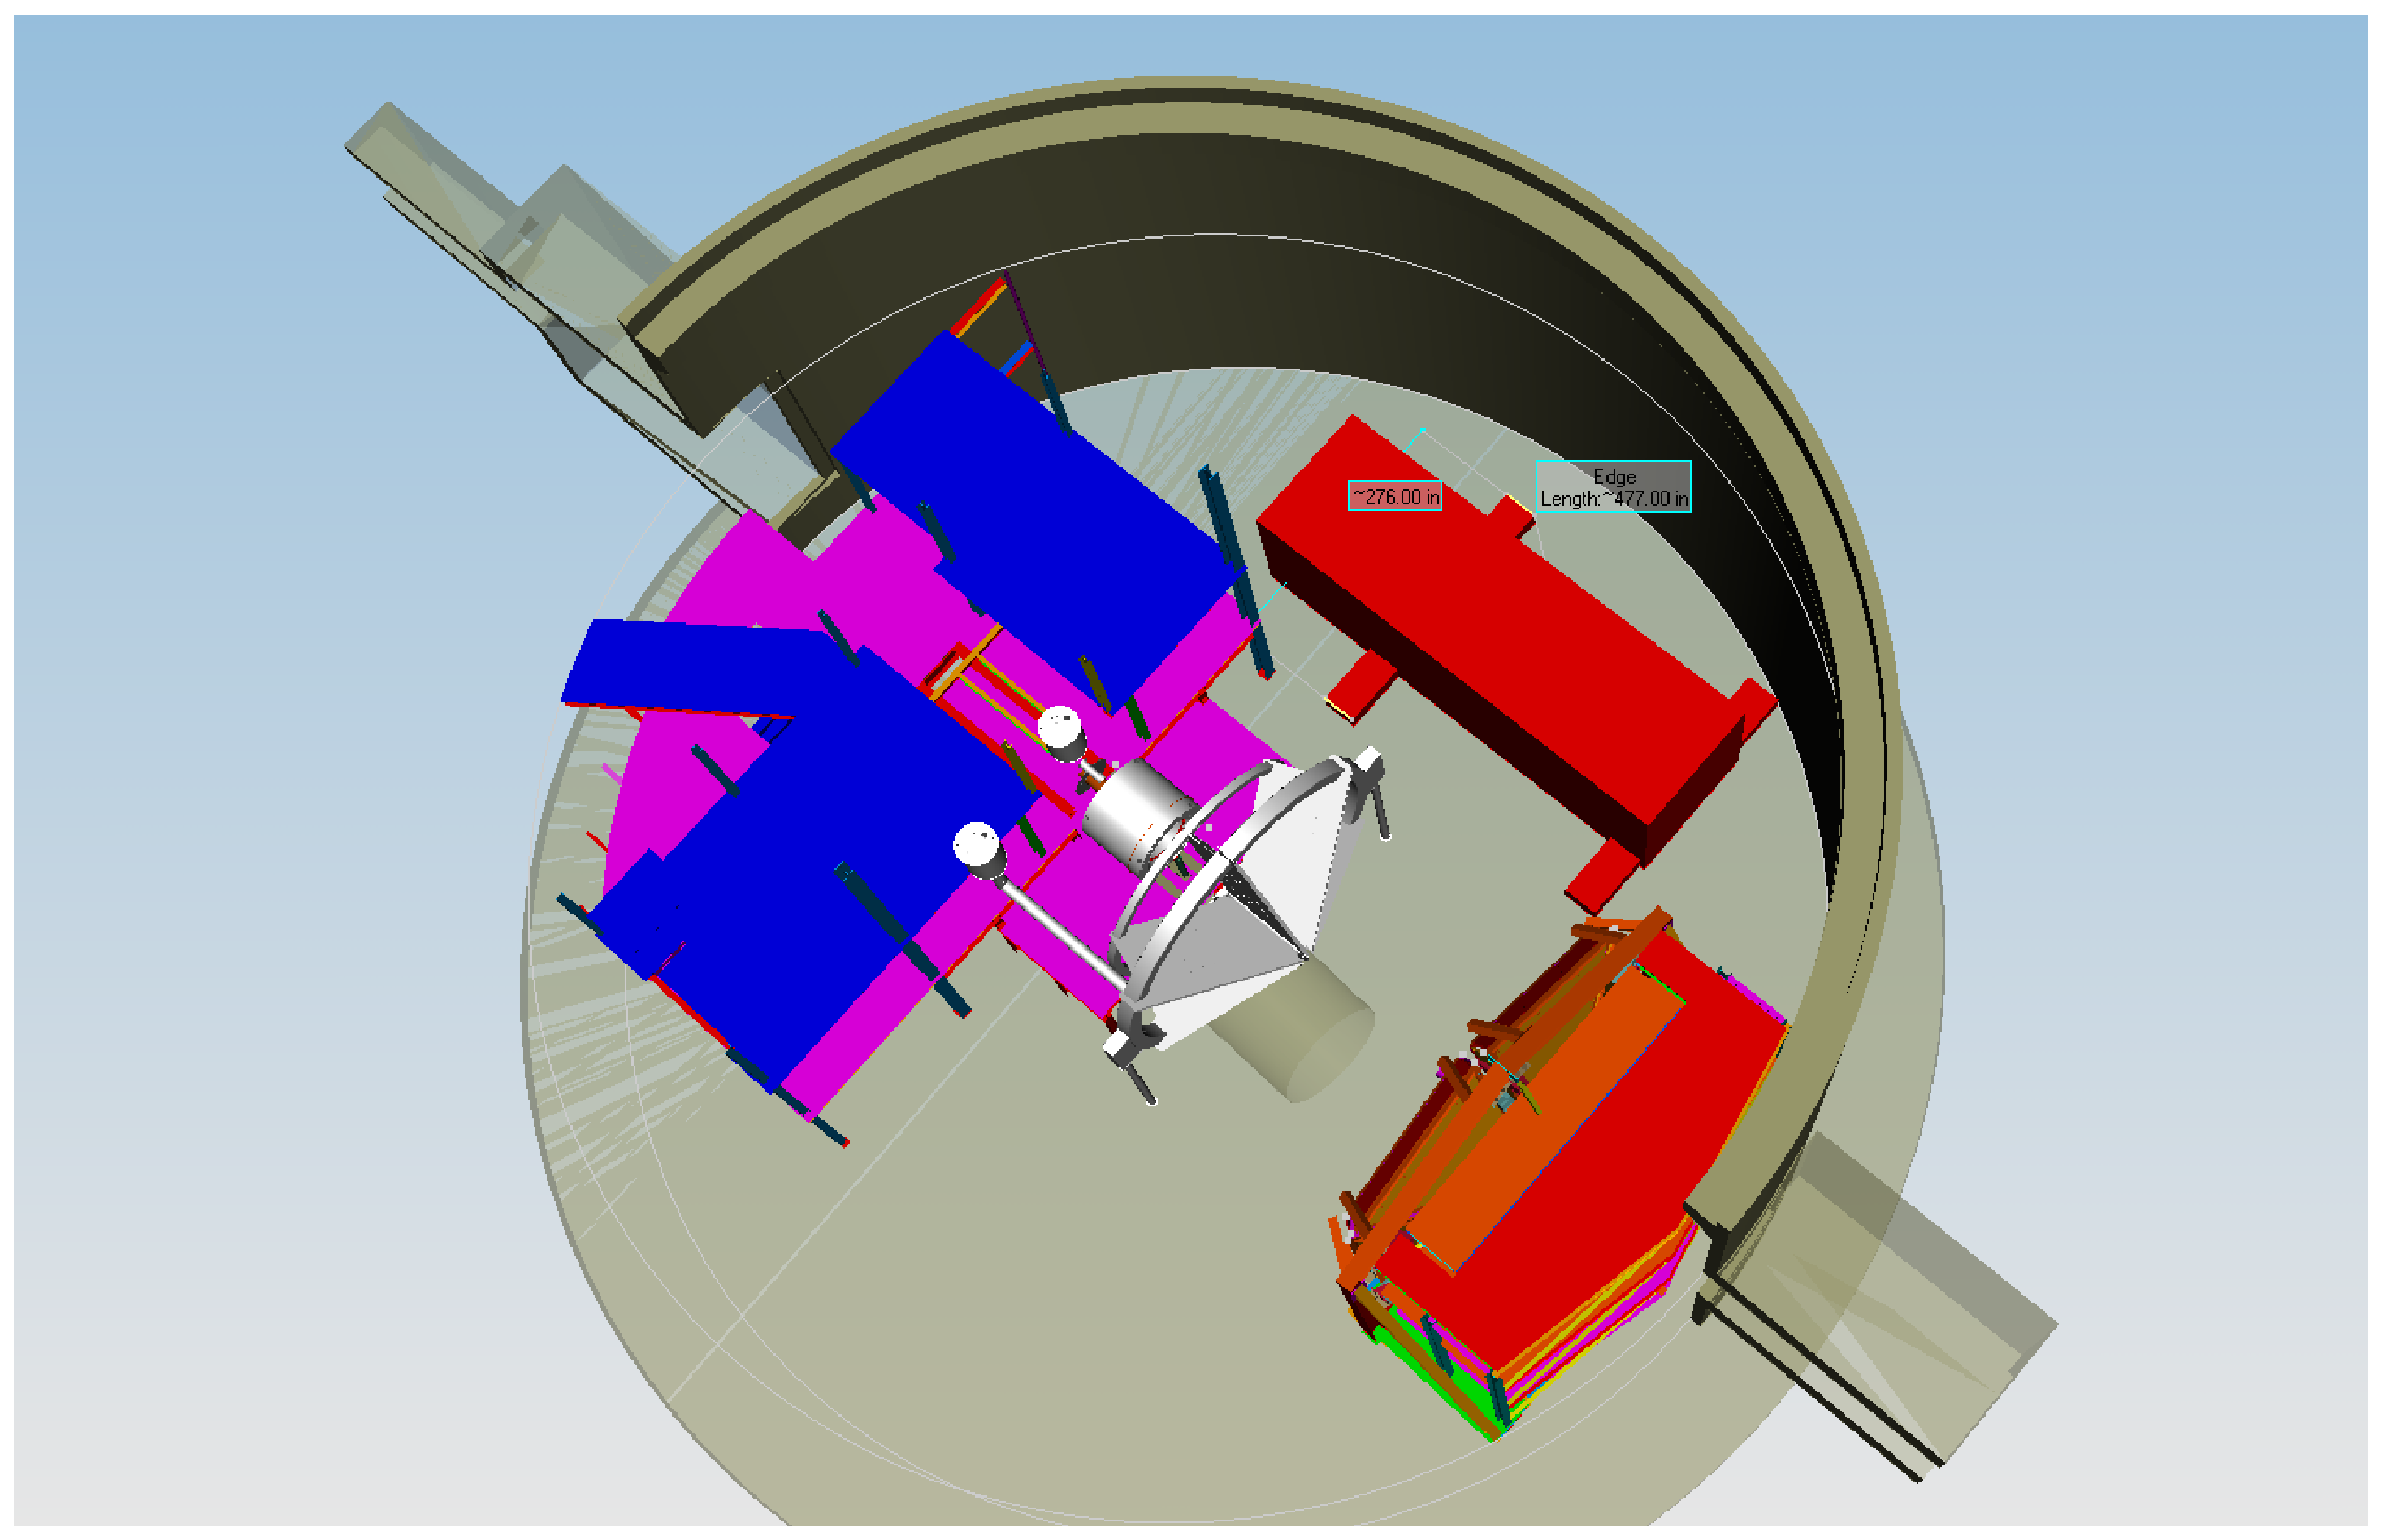
\includegraphics[width=0.6\textwidth]{CLAS12_view_37.eps}
\caption{\small{Overhead view of Hall~B showing the {\tt CLAS12}
configuration and the positioning of a mobile crane for installation
of the solenoid.  This plan will be used only if the final weight
of the solenoid is more than 20~tons.}}
\label{mobile}
\end{figure}
%%%%%%%%%%%%%%%%%%%%%%%%%%%%%%%%%%%%%%%%%%%%%%%%%%%%%%%%%%%%%%%%%%%%%%

\subsection{SVT}

The SVT system is an interesting case. It is so light that no cranes 
will be necessary to carry the load, but it is very fragile.  The 
current plan is to mount the SVT on an extension tube that is supported
from the solenoid.  The support fixture is also used for aligning the
detector.  The SVT is installed into the solenoid using the {\tt CLAS}
insertion cart.  Before installation, the SVT will be pre-aligned
on the beam line.

\section{Permanent Support Devices}

\subsection{Torus Support}

The torus will be mounted on a support stand that sits on the floor of 
Hall~B.  The magnet will be supported from three legs.  The support
system will be tied to Sub-level~1 of the Space Frame to increase the
stability of the system.

\subsection{Drift Chambers}

The three regions of drift chambers will be attached to the torus.  This 
is done to allow accurate, reliable, and repeatable positioning with respect 
to the magnetic field that is used for bending the charged particles.
A six link system (shown in Fig.~\ref{dc_links}) has been prototyped for 
this attachment system.  The prototype has been shown to have a 
reproducibility of 25~$\mu$m for chamber positioning.  The system has also 
been designed to allow for easy access to the individual chambers to 
facilitate repairs.

%%%%%%%%%%%%%%%%%%%%%%%%%%%%%%%%%%%%%%%%%%%%%%%%%%%%%%%%%%%%%%%%%%%%%%
\begin{figure}[htbp]
\centering
\includegraphics[width=0.6\textwidth]{r2_links.eps}
\caption{\small{Photograph of the link system installed in the
Region~2 drift chamber plywood prototype.  The link systems for
all 18 {\tt CLAS12} drift chambers will be of a similar design.}}
\label{dc_links}
\end{figure}
%%%%%%%%%%%%%%%%%%%%%%%%%%%%%%%%%%%%%%%%%%%%%%%%%%%%%%%%%%%%%%%%%%%%%%

\subsection{PCAL}

The pre-shower calorimeter will be supported from three points. The nose will 
have a docking ring similar to the drift chambers. The back two corners will 
have arms that reach from the Forward Carriage upstream, and attach to each 
sector.  These arms will have slots that allow for some misalignment of the 
brackets that must be welded to the Forward Carriage.

\subsection{Panel-2 FTOF}
 
FTOF panel-2 will be attached to the Forward Carriage on the outer hex ring. 
These panels will be hinged to allow them to be folded back such that 
they are clear of the other detectors.  A jack screw position arm will allow 
them to be moved in and out. It may be possible to re-use the jack screws 
from the {\tt CLAS} panel-4 TOFs.

\subsection{LTCC Arms}

The LTCC supports will be changed. The current support arms slide between 
the LTCC boxes. There are several good reasons to modify this support system.
This system has very little clearance and sometimes the installation or 
removal process results in making small leaks in the detector.  The space 
that the original arms take is very valuable and is needed for the PCAL 
phototube assemblies.  The current system requires that the LTCC come in 
parallel to the beam direction.  A different support system is being designed 
to allow the sectors to come in from other angles and this reduces the space 
required for installation.  The nominal design for the new support system
includes attachments at the nose and outer corners of each LTCC box.

\subsection{CTOF Supports} 
 
The central TOF will be supported from the solenoid cryostat.  Detailed
engineering and design work on this support is presently underway.

\section{Carts}

\subsection{Central Detector Cart}

The central detector includes the solenoid, central time-of-flight system, 
and the silicon vertex tracker.  It may in the future also include a central 
calorimeter.  These systems combine to a significant load for this cart. 
The estimated total weight is 40,000~lbs.  The cart must be designed to 
allow for alignment of the solenoid to the beam axis.  The current
design of the central detector cart is shown in Fig.~\ref{solenoidcart}.

%%%%%%%%%%%%%%%%%%%%%%%%%%%%%%%%%%%%%%%%%%%%%%%%%%%%%%%%%%%%%%%%%%%%%%
\begin{figure}[htbp]
\centering
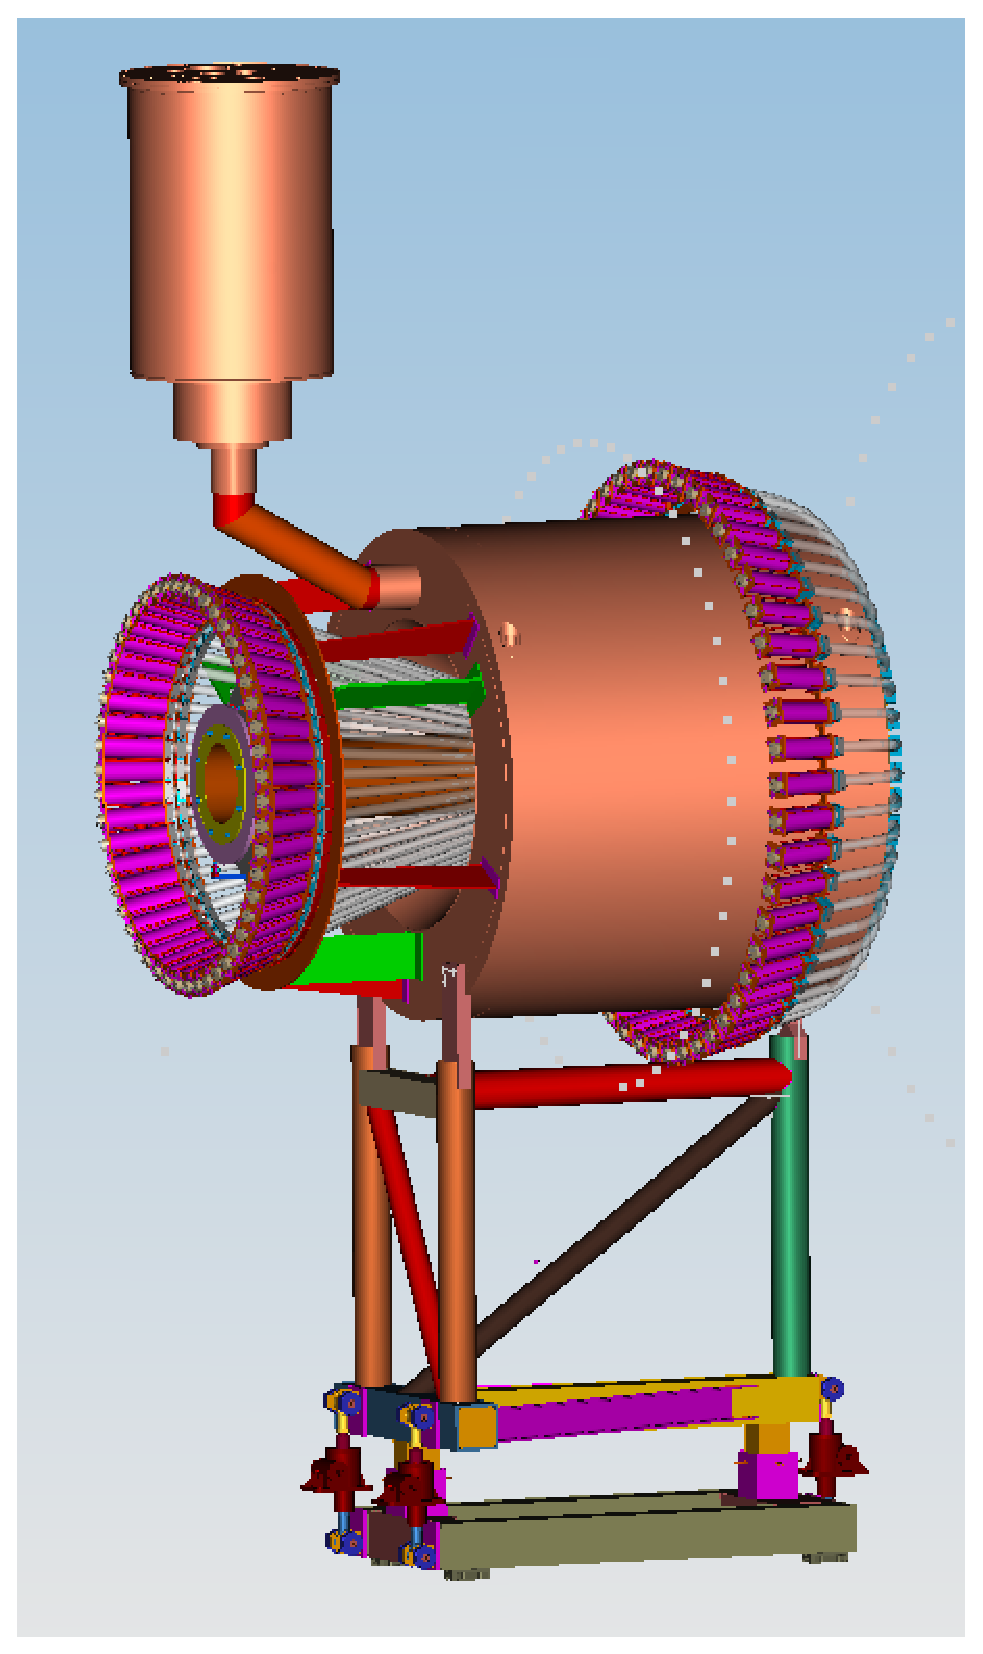
\includegraphics[width=0.6\textwidth]{solenoidcart.eps}
\caption{\small{{\tt CLAS12} central detector cart.
\label{solenoidcart}}}
\end{figure}
%%%%%%%%%%%%%%%%%%%%%%%%%%%%%%%%%%%%%%%%%%%%%%%%%%%%%%%%%%%%%%%%%%%%%%

\subsection{HTCC Beam Line Cart}

The HTCC weight is approximately 5000~lbs.  It will be supported from 
rails on the deck described in Section~\ref{sec:in_sf}.  It will have 
an alignment cart (see Fig.~\ref{htcc_cart}) that allows positioning of 
the detector to better than 0.5~mm. 

%%%%%%%%%%%%%%%%%%%%%%%%%%%%%%%%%%%%%%%%%%%%%%%%%%%%%%%%%%%%%%%%%%%%%%
\begin{figure}[htbp]
\centering
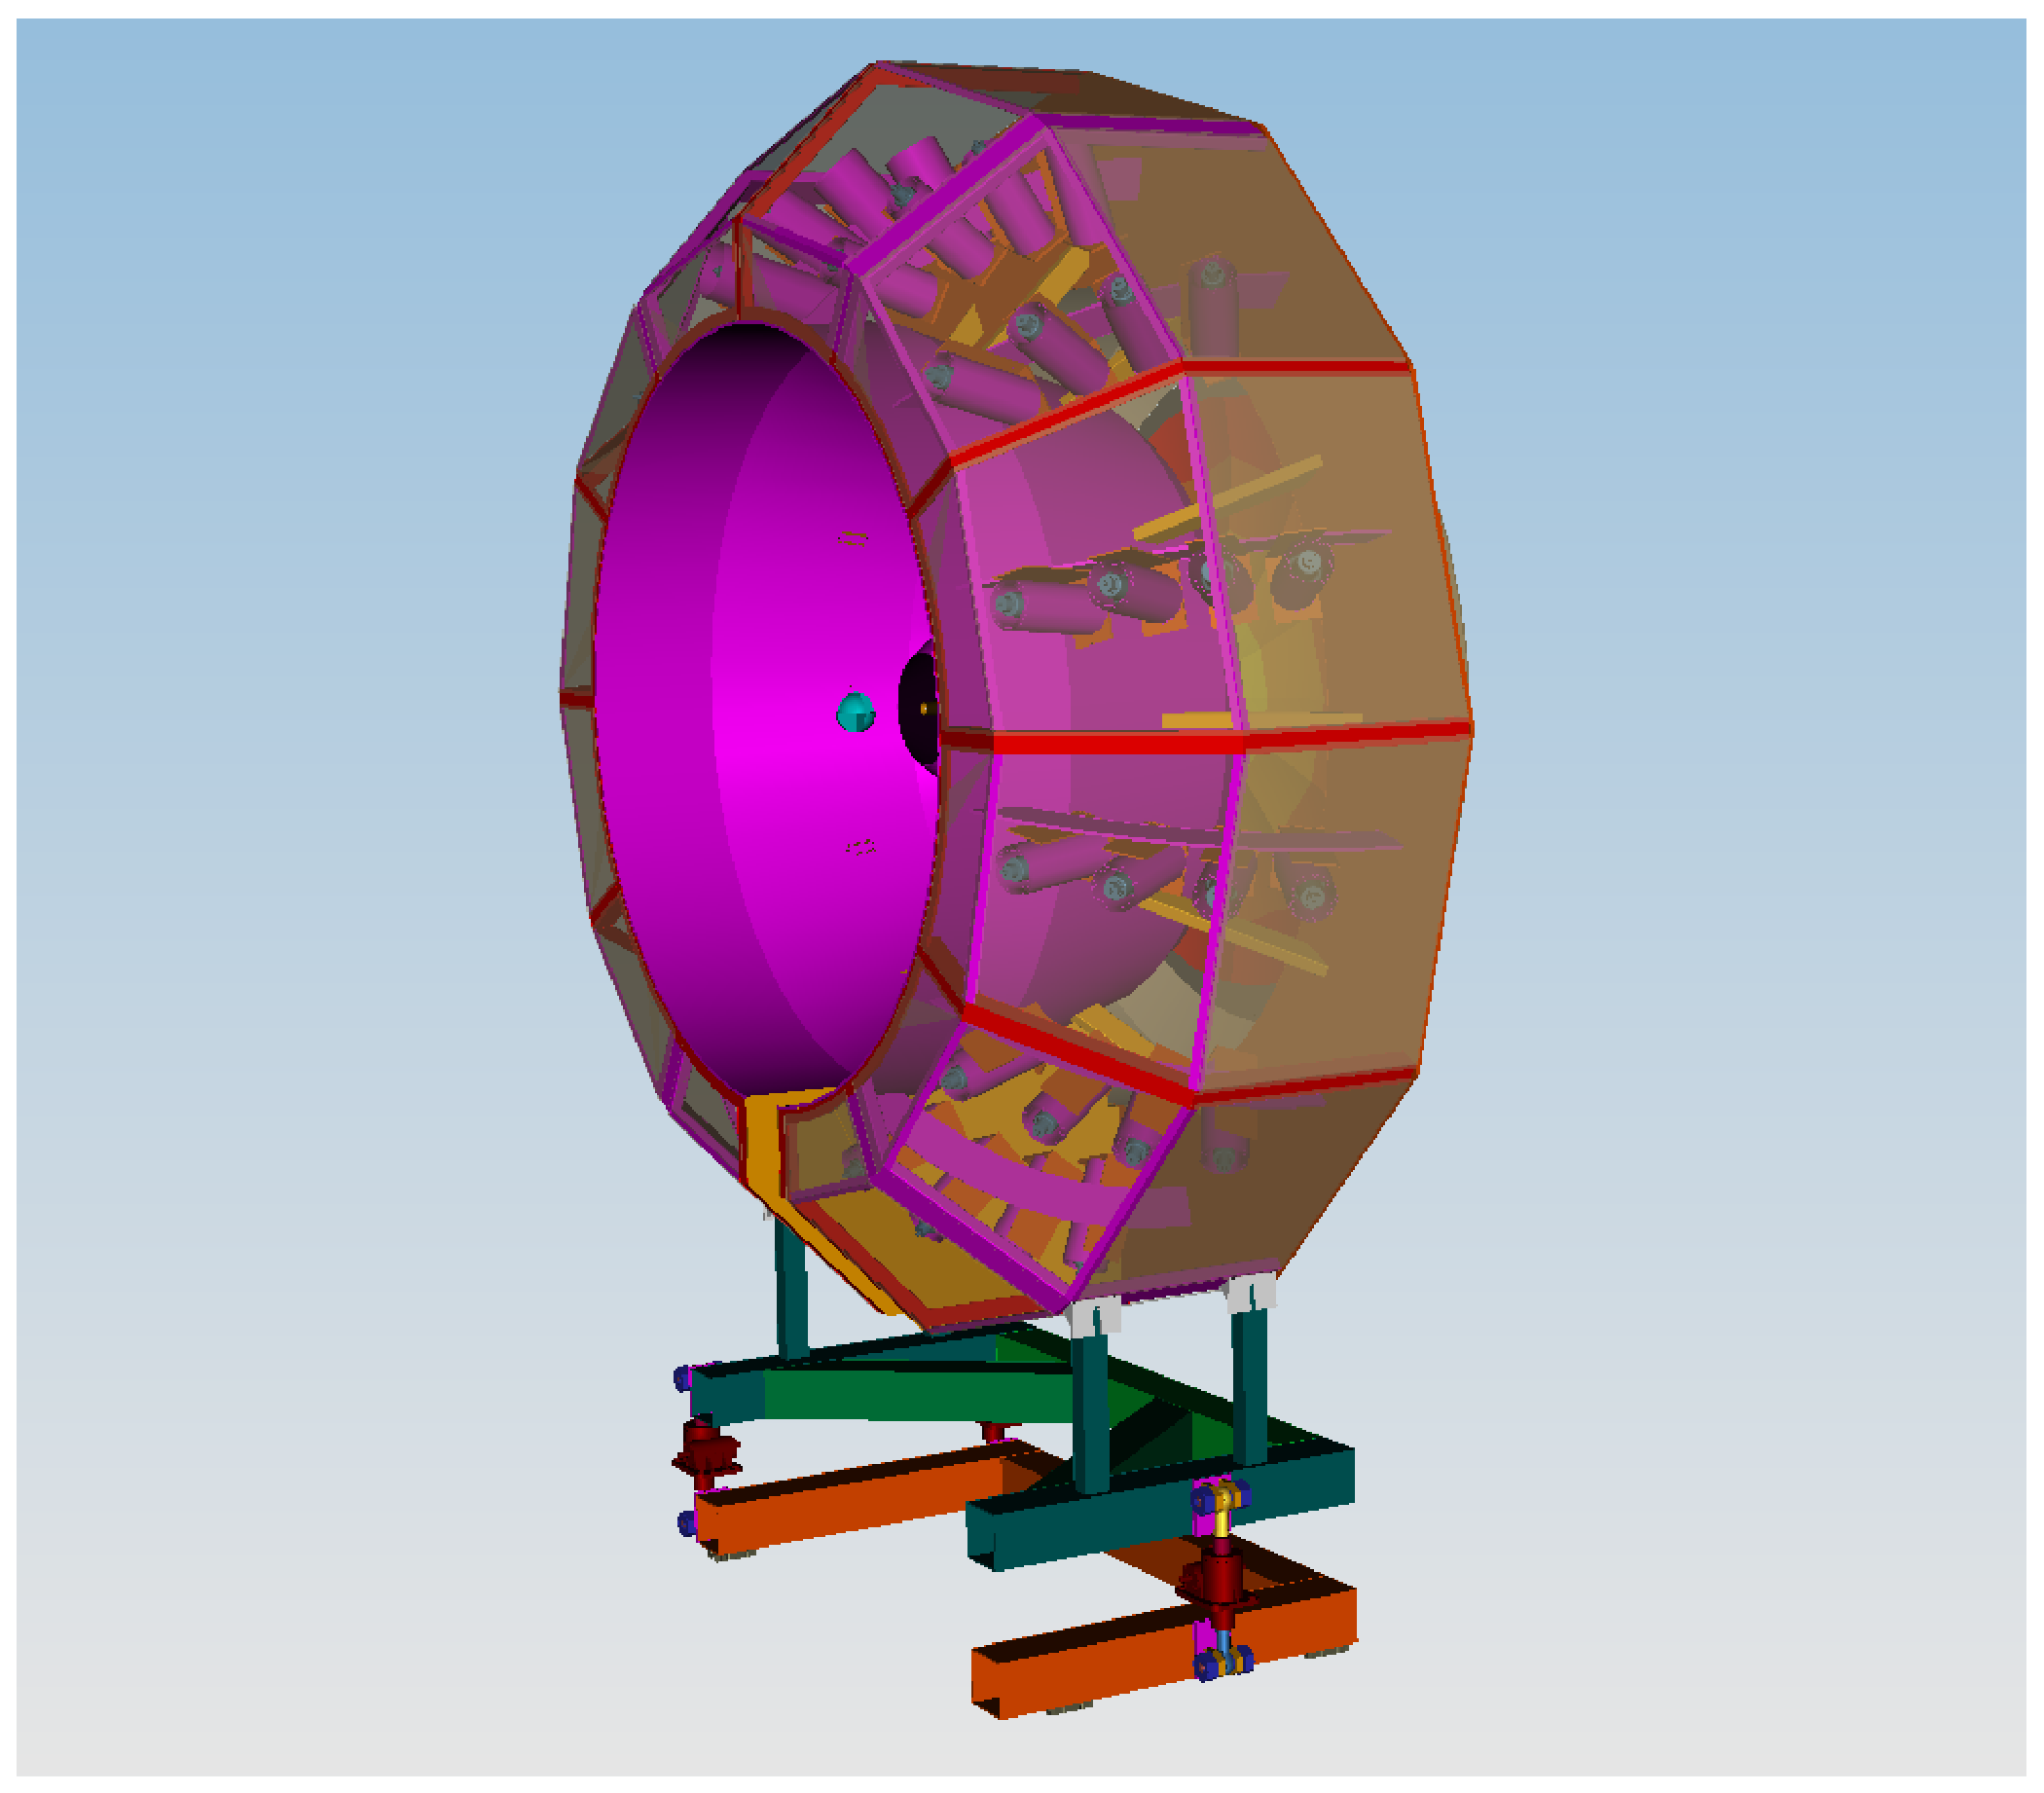
\includegraphics[width=0.6\textwidth]{htcc_cart.eps}
\caption{\small{{\tt CLAS12} HTCC on its installation cart.
\label{htcc_cart}}}
\end{figure}
%%%%%%%%%%%%%%%%%%%%%%%%%%%%%%%%%%%%%%%%%%%%%%%%%%%%%%%%%%%%%%%%%%%%%%

\subsection{Polarized Target Cart}

The polarized target will have a cart similar to the Frost target that was 
designed and built for {\tt CLAS}.  Fig.~\ref{poltarget} shows a
schematic diagram showing the polarized target assembly on its installation
cart.

%%%%%%%%%%%%%%%%%%%%%%%%%%%%%%%%%%%%%%%%%%%%%%%%%%%%%%%%%%%%%%%%%%%%%%
\begin{figure}[htbp]
\centering
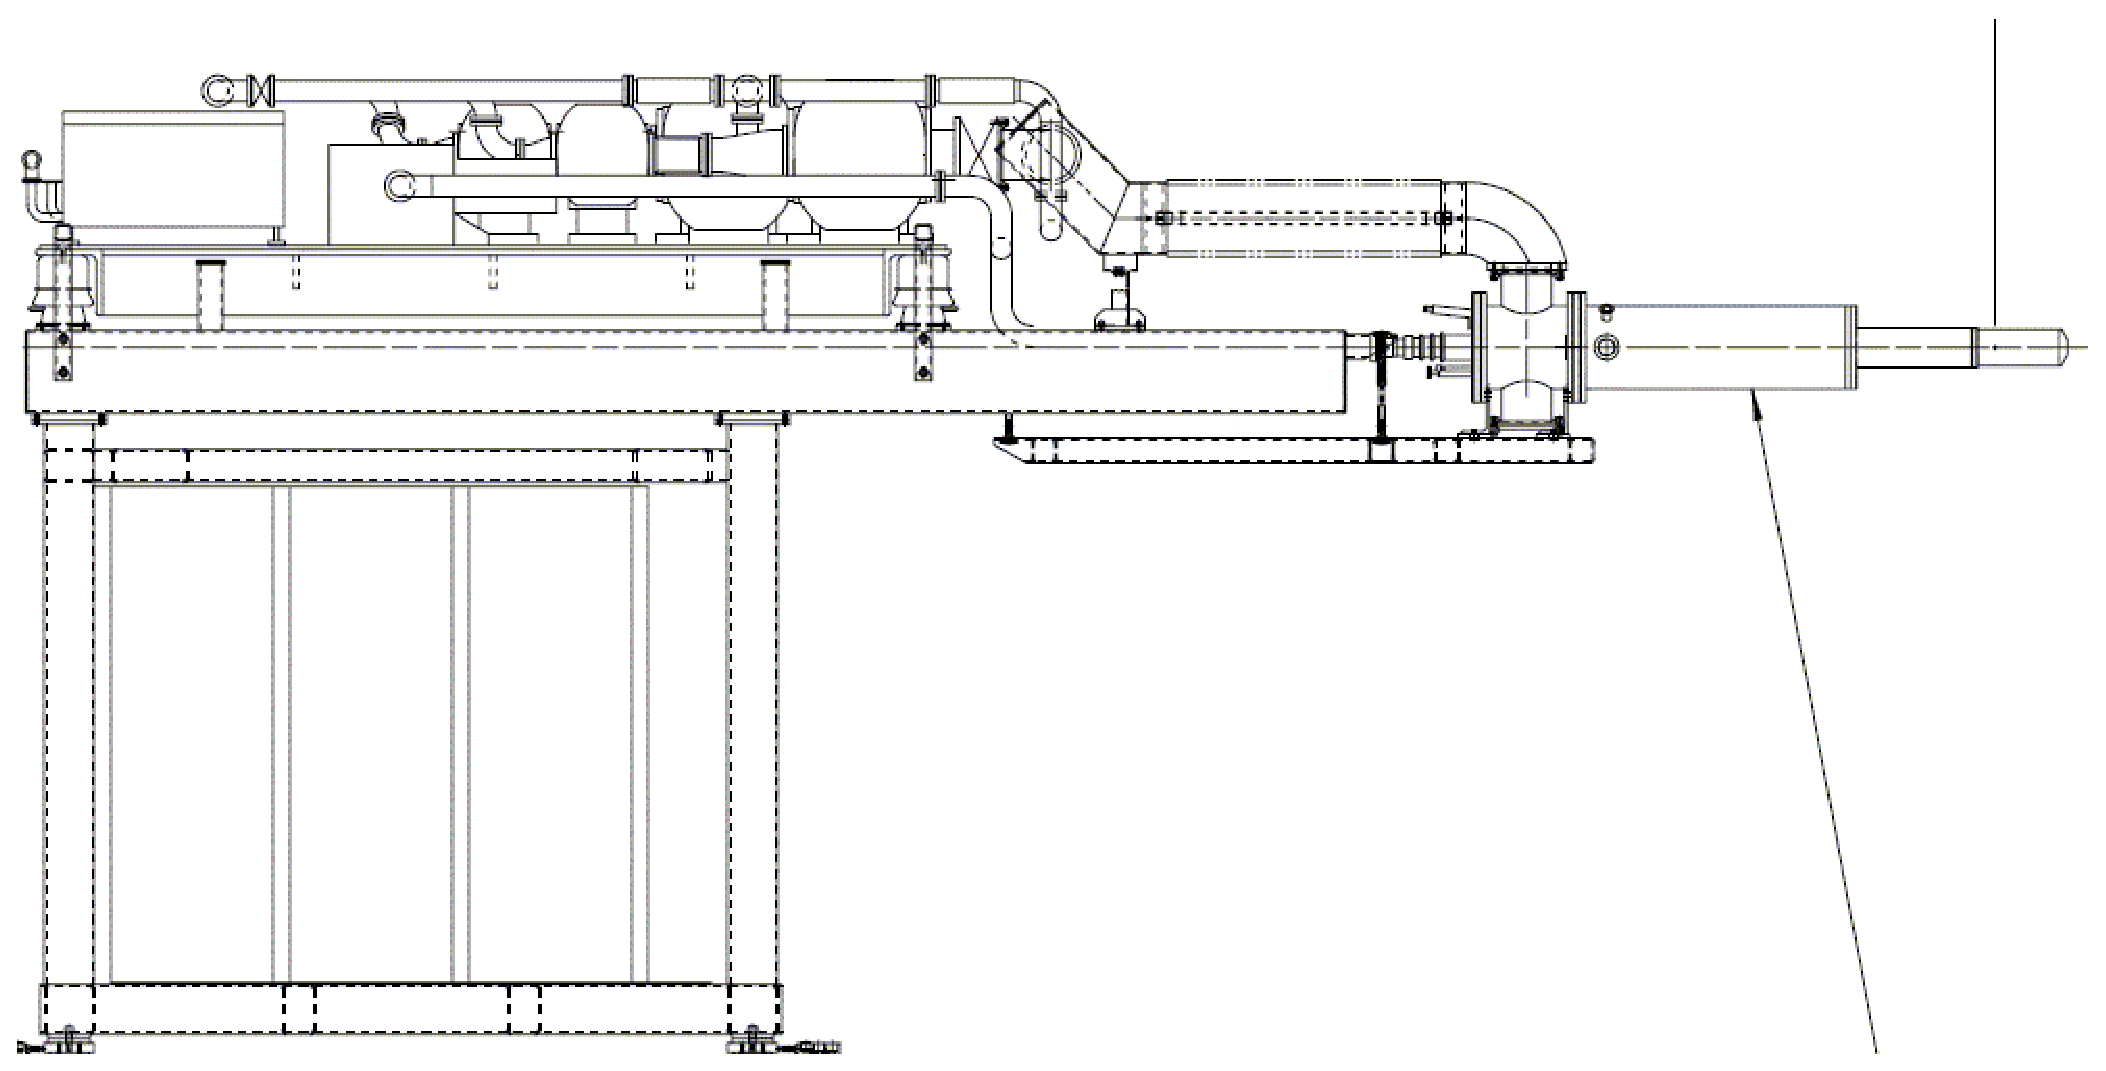
\includegraphics[width=0.6\textwidth]{polarizedtarget.eps}
\caption{\small{Schematic of the polarized target assembly on its
installation cart.}}
\label{poltarget}
\end{figure}
%%%%%%%%%%%%%%%%%%%%%%%%%%%%%%%%%%%%%%%%%%%%%%%%%%%%%%%%%%%%%%%%%%%%%%

\section{Utilities}

\subsection{Cryogenic Distribution Can and U-tubes}

The cryogenic distribution can will be installed in the same location as 
the {\tt CLAS} torus service module.  The supply transfer line will need no 
modifications.  The new can will have 3 sets of 4~K bayonets, 1 set of 
15~K bayonets, and 3 sets of liquid-nitrogen bayonets.  Fig.~\ref{cryoschem}
shows the planned cryogenic cooling distribution schematic.

%%%%%%%%%%%%%%%%%%%%%%%%%%%%%%%%%%%%%%%%%%%%%%%%%%%%%%%%%%%%%%%%%%%%%%
\begin{figure}[htbp]
\centering
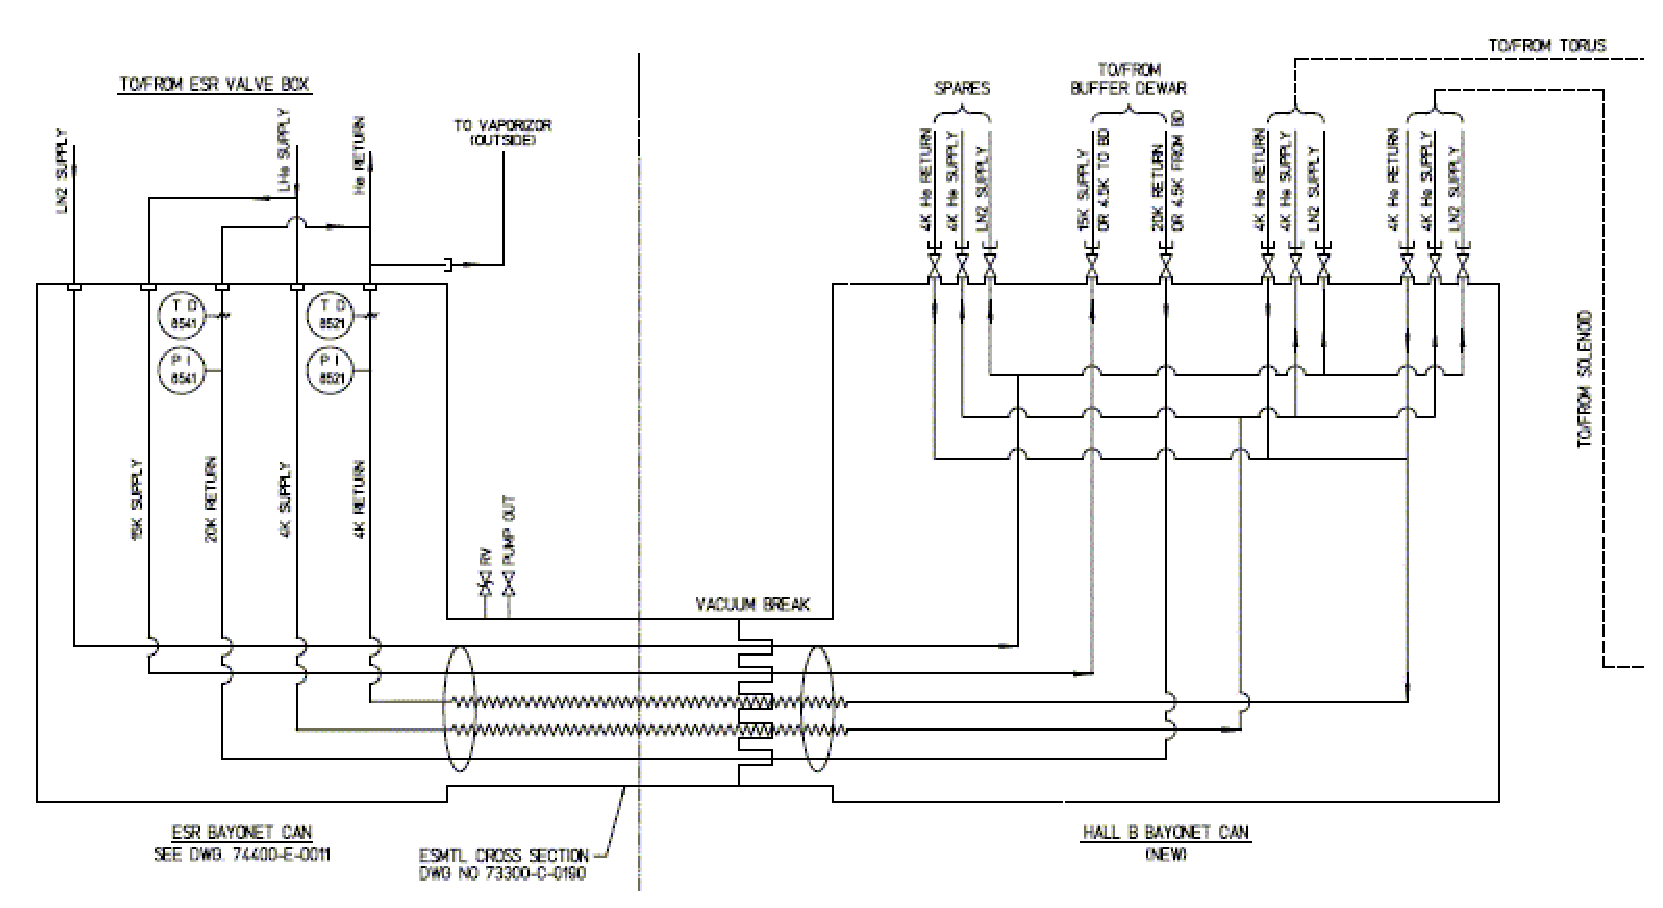
\includegraphics[width=0.6\textwidth]{cryoschematic.eps}
\caption{\small{Cryogenic cooling distribution schematic.}}
\label{cryoschem}
\end{figure}
%%%%%%%%%%%%%%%%%%%%%%%%%%%%%%%%%%%%%%%%%%%%%%%%%%%%%%%%%%%%%%%%%%%%%%

\subsection{HVAC Cooling Power}

Hall B uses a chilled-water cooling system for meeting the HVAC load 
requirements.  The present system has four compressors, and during normal 
operations, the load varies such that only 2 or 3 are needed.  The 
upgraded {\tt CLAS12} will have more electronics.  

\subsection{LCW}

No change in the system will be necessary to accommodate the Hall B loads. 
Some minor plumbing will be necessary to connect the new magnet power 
supplies. 

\subsection{Electrical Service}

No capacity increase in the electrical service that exists for {\tt CLAS}
will be required for {\tt CLAS12}.  Only minor circuit installation and 
relocation is currently expected. 

\subsection{SVT and IC Cooling}

The SVT and IC detectors will each have a small chiller system installed 
to remove heat from the electronics.

\subsection{Cable Trays}

Significant cable tray work will be necessary for {\tt CLAS12}. Most of 
this will be the cables for the three regions of drift chambers. 

\section{Survey}

JLab has a survey and alignment group that provides services lab-wide.
Their tooling includes two Faro Laser Tracking Tools, models SI and X.
These are used for alignment and to make {\it as found} measurements of
systems throughout JLab. All detectors and beam line devices are
fiducialized prior to being installed into the accelerator or one of
the Halls.  Depending on the design of the alignment system, large
detectors can be aligned to accuracies better than 200~$\mu$m and 
knowledge of the location can be ascertained to 50~$\mu$m when necessary. 
Each detector will have tooling ball mounts that are used to facilitate 
both the fiducialization and alignment. Support connections will be 
designed to allow precise alignment for detectors where this type of 
alignment is critical, e.g. the drift chambers and targets.  For other 
detectors such as the LTCC, FTOF, and PCAL, where alignment is not
critical, much less precise systems will be used.

\section{Safety}

All persons that will work on {\tt CLAS12} detectors on site will receive 
job specific training. ISM (integrated safety management) principles will 
be used. Resources from the EHS\&Q division will be brought to bear to help 
developing any new procedures that are not documented in the EHS\&Q manual. 
Specific fabrication and installation procedures will be developed for each 
detector system by the lead engineers and physicists. All lifting devices 
will be load tested prior to use and specific lift plans will be developed. 
The determination of what lifts will be done by who will be done by a rigger 
with Master Rigger Qualification. 
